\documentclass[tikz,border=3mm,multi=tikzpicture]{standalone}
\usepackage[utf8]{inputenc}
\usepackage[T1]{fontenc}
\usepackage{helvet}
\renewcommand{\familydefault}{\sfdefault}
\usepackage{tikz}
\usetikzlibrary{arrows.meta,positioning,patterns}
\begin{document}

\tikzset{every node/.append style={font=\sffamily\small}}

% TikZ 1
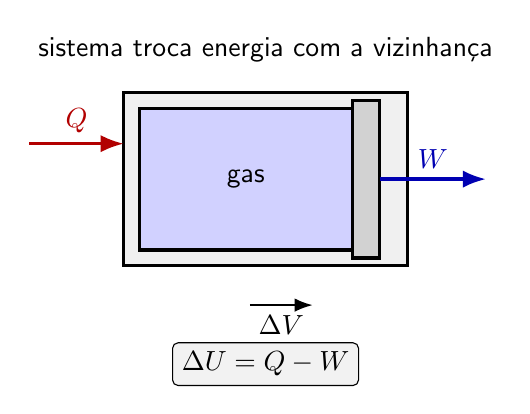
\begin{tikzpicture}[>=Latex]
  \draw[very thick,fill=gray!12] (-1.8,-1.1) rectangle (1.8,1.1);
  \draw[very thick,fill=blue!18] (-1.6,-0.9) rectangle (1.1,0.9);
  \draw[very thick,fill=gray!35] (1.1,-1.0) rectangle (1.45,1.0);
  \node at (-0.25,0) {gas};
  \draw[very thick,->,red!70!black] (-3,0.45) -- (-1.8,0.45) node[midway,above] {$Q$};
  \draw[very thick,->,blue!70!black] (1.45,0) -- (2.8,0) node[midway,above] {$W$};
  \draw[->,thick] (-0.2,-1.6) -- (0.6,-1.6) node[midway,below] {$\Delta V$};
  \node[align=center] at (0,1.65) {sistema troca energia com a vizinhança};
  \node[draw,rounded corners=2pt,fill=gray!10,align=center] at (0,-2.35)
    {$\Delta U = Q - W$};
\end{tikzpicture}

% TikZ 2
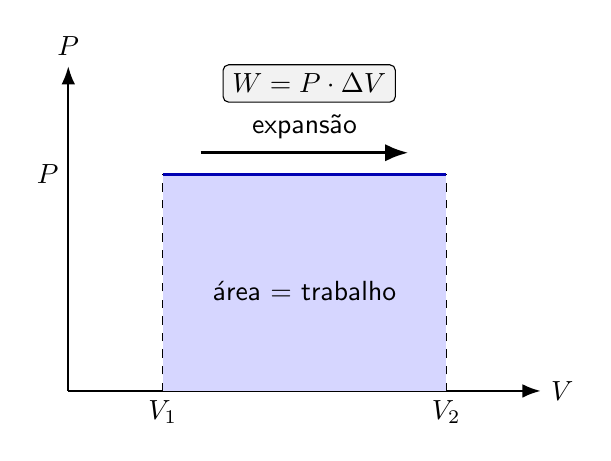
\begin{tikzpicture}[x=1.2cm,y=1.1cm,>=Latex]
  \draw[->,thick] (0,0) -- (5,0) node[right] {$V$};
  \draw[->,thick] (0,0) -- (0,3.75) node[above] {$P$};
  \fill[blue!16] (1,0) -- (1,2.5) -- (4,2.5) -- (4,0) -- cycle;
  \draw[very thick,blue!70!black] (1,2.5) -- (4,2.5);
  \draw[dashed] (1,0) -- (1,2.5);
  \draw[dashed] (4,0) -- (4,2.5);
  \node[below] at (1,0) {$V_1$};
  \node[below] at (4,0) {$V_2$};
  \node[left] at (0,2.5) {$P$};
  \node[align=center] at (2.5,1.15) {área = trabalho};
  \draw[very thick,->] (1.4,2.75) -- (3.6,2.75);
  \node[above] at (2.5,2.8) {expansão};
  \node[draw,rounded corners=2pt,fill=gray!10,align=center] at (2.55,3.55)
    {$W=P\cdot\Delta V$};
\end{tikzpicture}

% TikZ 3
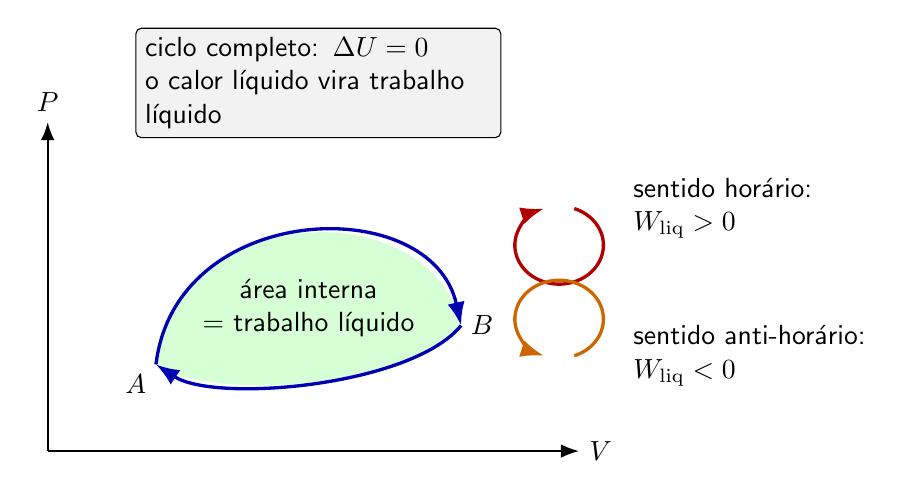
\begin{tikzpicture}[x=1.25cm,y=1.1cm,>=Latex]
  \draw[->,thick] (0,0) -- (5.4,0) node[right] {$V$};
  \draw[->,thick] (0,0) -- (0,3.8) node[above] {$P$};

  \fill[green!16] (1.1,1) .. controls (1.3,2.9) and (3.9,3.0) .. (4.2,1.45)
    .. controls (3.7,0.75) and (1.7,0.55) .. (1.1,1) -- cycle;

  \draw[very thick,blue!70!black,->]
    (1.1,1) .. controls (1.3,2.9) and (3.9,3.0) .. (4.2,1.45);
  \draw[very thick,blue!70!black,->]
    (4.2,1.45) .. controls (3.7,0.75) and (1.7,0.55) .. (1.1,1);

  \node[below left] at (1.1,1) {$A$};
  \node[right] at (4.2,1.45) {$B$};
  \node[align=center] at (2.65,1.65) {área interna\\$=$ trabalho líquido};

  \node[draw,rounded corners=2pt,fill=gray!10,align=left,text width=4.4cm]
    at (2.75,4.25)
    {ciclo completo: $\Delta U=0$\\o calor líquido vira trabalho líquido};

  \draw[very thick,->,red!70!black] (5.35,2.8) arc[start angle=70,end angle=-250,radius=.45];
  \node[align=left,right] at (5.85,2.8) {sentido horário:\\$W_{\mathrm{liq}}>0$};

  \draw[very thick,->,orange!80!black] (5.35,1.1) arc[start angle=-70,end angle=250,radius=.45];
  \node[align=left,right] at (5.85,1.1) {sentido anti-horário:\\$W_{\mathrm{liq}}<0$};
\end{tikzpicture}

\end{document}
